\documentclass[11pt]{article}
\usepackage[margin=1in]{geometry}
\usepackage{amsmath}
\usepackage{booktabs}
\usepackage{graphicx}
\usepackage{hyperref}
\title{Result 3.0: Explicit Finite Spin-Chain Hamiltonian for the SOC Workbench}
\author{}
\date{\today}
\begin{document}
\maketitle

\section{Purpose of the test}
This result tests whether the phenomenological nearest-neighbour spin-correlation input used in the projected bright--dark SOC model can be replaced by an explicit finite $S=1/2$ spin-chain Hamiltonian. The working hypothesis is that the spin sector can be solved independently to obtain
\begin{equation}
C_1(T,B)=\left\langle \mathbf S_i\cdot\mathbf S_{i+1}\right\rangle_{T,B},
\end{equation}
and that this value can then enter the same projected optical coupling used in the Step 3 dynamic phonon model.

\section{Physical model}
The spin Hamiltonian implemented in the workbench is
\begin{equation}
H_{\rm spin}=\sum_i J_i(T,B)\mathbf S_i\cdot\mathbf S_{i+1}+J_2\sum_i\mathbf S_i\cdot\mathbf S_{i+2}+g\mu_B B\sum_i S_i^z,
\end{equation}
with
\begin{equation}
J_i(T,B)=J\left[1+(-1)^i\delta(T,B)\right].
\end{equation}
The finite chain uses $N=6$ spins and open boundary conditions. The optical sector is kept aligned with the Step 3 notebook:
\begin{equation}
H_{\rm opt}=H_{\rm orb}\otimes I_{\rm ph}+\omega_Q I_{\rm orb}\otimes a^\dagger a+V_{BD}L_{BD}\otimes I_{\rm ph}+g_Q L_{BD}\otimes(a+a^\dagger).
\end{equation}
Here $L_{BD}=|B\rangle\langle D|+|D\rangle\langle B|$ and
\begin{equation}
V_{BD}=V_0+\lambda_\delta\delta(T,B)+\lambda_C C_1(T,B).
\end{equation}
The full spin Hilbert space is not tensored into the Liouville spectroscopy calculation in this result; it is used to compute $C_1$ exactly for the projected optical model.

\section{Calculation definitions}
The workbench is controlled by a single Python dictionary, \verb|model_params|, which contains all physical and numerical model parameters for the active calculation. Rephasing spectra were evaluated on $\omega_1<0$, $\omega_3>0$, while unrephasing spectra were evaluated separately on $\omega_1>0$, $\omega_3>0$.

\section{Active parameter set and acceptance criteria}
\begin{center}
\begin{tabular}{lcccc}
\toprule
Output stem & $T$ (K) & $B$ (T) & $N_{\rm spin}$ & Active spin source \\
\midrule
SOC\_workbench & 7.0 & 0.0 & 6 & exact $H_{\rm spin}$ \\
\bottomrule
\end{tabular}
\end{center}
Acceptance criteria: the spin Hamiltonian must be Hermitian and have dimension $2^N$; every run must produce linked raw arrays and the six mandatory real, imaginary, and absolute rephasing/unrephasing figures; the rephasing and unrephasing frequency quadrants must be distinct; and $C_1$ must be computed from the explicit spin Hamiltonian and injected into $V_{BD}$.

\section{Numerical results}
The generated metrics are stored in \verb|Analysis/step03__spin_chain_exact_metrics.csv|. The main derived values are:
\begin{center}
\begin{tabular}{lrrrrrr}
\toprule
Output & $T$ & $B$ & $\delta$ & $C_1$ & $V_{BD}$ & Reph. $|S|$ int. \\
\midrule
SOC\_workbench & 7.0 & 0.0 & 0.00707 & -0.49863 & 0.02267 & 4.854e+02 \\
\bottomrule
\end{tabular}
\end{center}
\begin{figure}[h]
\centering
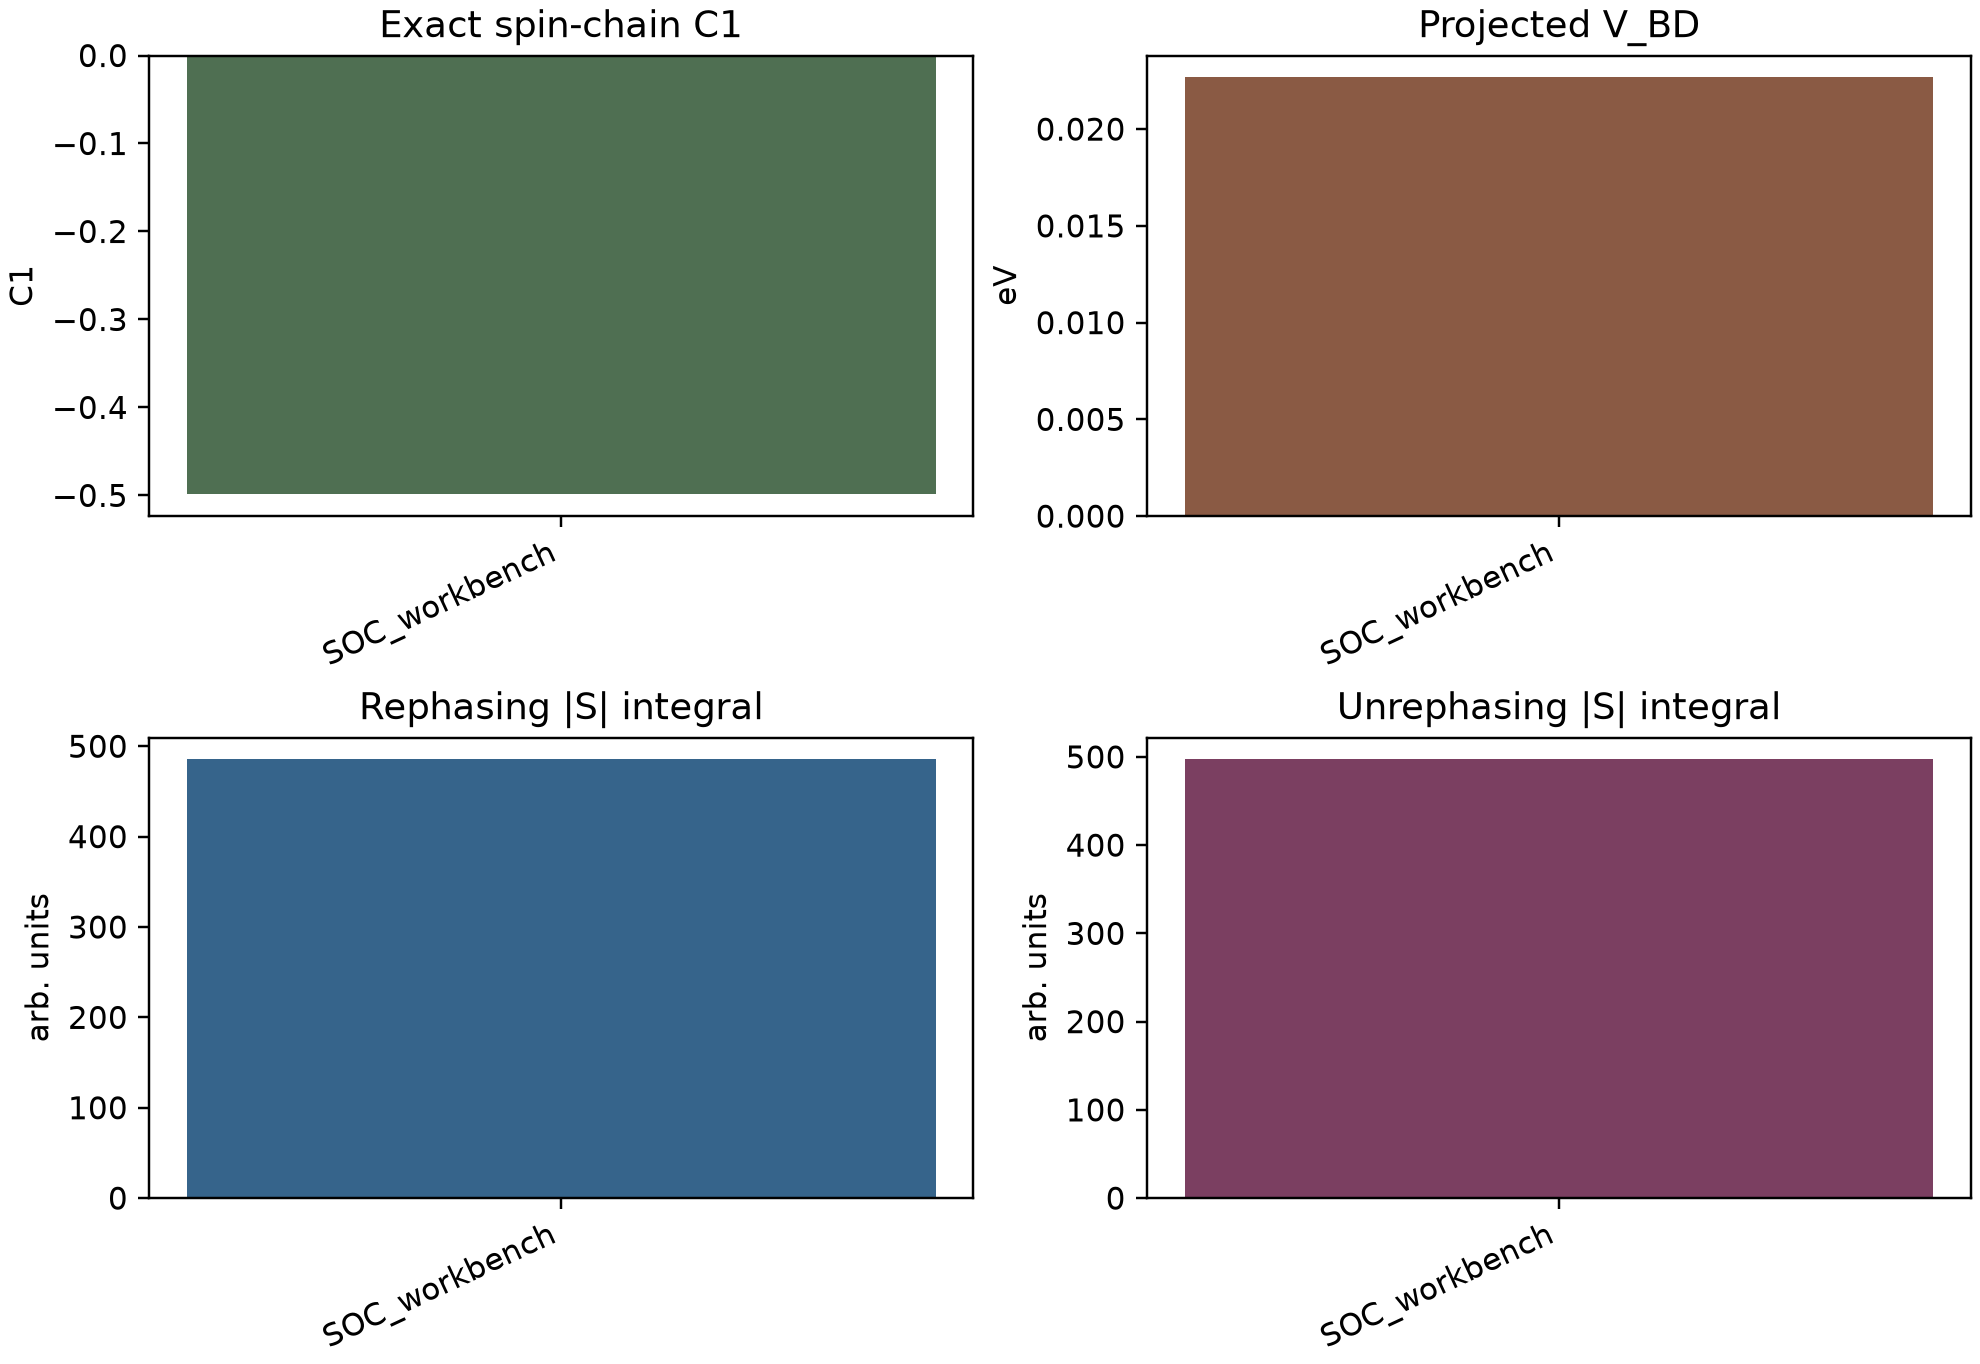
\includegraphics[width=0.92\linewidth]{../Analysis/step03__spin_chain_exact_comparison.png}
\caption{Exact spin-chain $C_1$, projected $V_{BD}$, and integrated 2D response metrics for the active parameter dictionary.}
\end{figure}

\section{Validation outcome}
The validation details are saved in \verb|Analysis/step03__spin_chain_exact_validation_outcome.txt|. All acceptance criteria are evaluated from raw arrays and generated file existence. The evidence supports the limited conclusion that this workbench now contains a real finite-chain $H_{\rm spin}$ and uses its thermal nearest-neighbour correlation in the projected optical SOC model. It does not yet validate a full tensor-product spin--orbital Liouville calculation.
\end{document}
